\documentclass[leqno, 11pt]{article}

\usepackage{lmodern}
\usepackage[scaled]{beramono}
\usepackage[T1]{fontenc}
\usepackage{amssymb}
\usepackage{amsmath}
\usepackage{hyperref}
\hypersetup{%
  colorlinks=true,
  linkcolor=magenta,
  filecolor=magenta,
  urlcolor=magenta
}

\usepackage[margin=1in]{geometry}
\usepackage{listings}
\usepackage{graphicx}
\usepackage{caption}
\captionsetup{%
  width=1.0\linewidth,
  justification=centering
}
\usepackage{float}

\usepackage{verbatimbox}  % center \thebox

% Better `@' symbol
\newcommand{\at}{\mbox{}{\fontfamily{ptm}\selectfont @}\mbox{}}

\newcommand\blfootnote[1]{%
  \begingroup
    \renewcommand\thefootnote{}\footnote{#1}
    \addtocounter{footnote}{-1}
  \endgroup
}

%\graphicspath{"/home/brandon/Desktop/IFT_194/labs/photos"}

\usepackage{xcolor}
\definecolor{javacommentscolor}{HTML}{646464}
\definecolor{javakeywordscolor}{HTML}{7F0055}
\definecolor{javastringscolor}{HTML}{2A00FF}

\lstset{%
  basicstyle=\scriptsize\ttfamily, % code to be displayed as monospace
  breaklines=true,
  %frame=b
  commentstyle=\color{javacommentscolor},
  keywordstyle=\color{javakeywordscolor},
  stringstyle=\color{javastringscolor},
  showstringspaces=false,  % do not show string spaces character
  tabsize=4,  % change tabs to spaces
  keywordsprefix={@},  % capture method annotations and doctools
  %showtabs=true,
  %tab=|
}

\newcommand{\centeredimage}[2]{%
  \begin{center}
    \includegraphics[scale=#1]{#2}
  \end{center}
}

\title{\vspace{6ex}The Java Programming Structure\\
  \Large IFT 194: HW 1}
\author{Brandon Doyle\\
\href{mailto:bdoyle@asu.edu}{bdoyle5\at{}asu.edu}\\
1215232174\\[1em]
Dr. Usha Jagannathan\\
\href{mailto:Usha.Jagannathan@asu.edu}{Usha.Jagannathan\at{}asu.edu}}

\setlength{\parindent}{0em}
\setlength{\parskip}{0.5em}

\begin{document}
\begin{titlepage}
\clearpage\maketitle
\thispagestyle{empty}
\end{titlepage}
\blfootnote{View the source of this document on \href{https://github.com/bjd2385/IFT_194_labs/blob/master/\jobname.tex}{GitHub}.}
\section*{Reading Questions}
\begin{enumerate}
  \item According to the reading, the original name of the Java programming language was ``Oak.''
  \item The author of the reading, Michael O'Connel, made the claim that ``... the solution preceeded the problem'' regarding the creation of Java. In this statement, the ``problem'' arose in mid-1994 when the Internet's popularity began growing. As Gosling says, there was a need for a ``really cool browser,'' which is an application that should be architecture-neutral, real-time, and secure. These are all qualities that had been built into Java since 1991.
  \item The creator of Java is James Gosling. The author also mentions Patrick Naughton, who was the ``project lead on Sun's OpenWindows user environment before joining the secret Green team,'' which was the team name for a consumer electronics effort at Sun Microsystems in the 1990s. Gosling's contributions to the team were usually to solve ``tooling'' problems that required extensive programming. Gosling had already, by that time, produced a number if interesting projects, such as the first implementation of the Emacs text editor in pure C (I actually have \href{https://www.gnu.org/software/emacs/}{GNU's Emacs} installed on my system now).
  \item The creators' motivations in writing Java were to make the language platform-neutral for consumers. Today there are a large number of different processors and architectures, even more-so than there were in the `90s. For example, the text also states that the goal was to ``build a system that would let us do a large, distributed, heterogeneous network of consumer electronic devices all talking to each other.''
  \item Java was spun into the web when Jonathan Payne wrote a web browser called WebRunner in Java. This allowed developers to write applications in the browser.
  \item The original target market for Java was consumer electronics. Java was created to solve the development issues programmers were having with creating systems running on different platforms (operating systems and architectures) that could communicate with each other. Languages (like Scala) that run on the JVM are platform independent.
\end{enumerate}
\section*{Textbook Exercises}
\subsection*{1.14}
According to the text and the \href{https://docs.oracle.com/javase/specs/jls/se10/html/jls-3.html#jls-3.7}{Java SE10 language specification}, there are two types of comments, including
\begin{enumerate}
  \item end-of-line comments, denoted by `\texttt{//}', and
  \item traditional comments, denoted by `\texttt{/*}...\texttt{*/}'.
\end{enumerate}
End-of-line comments delimit text on a single line that is to be ignored by the compiler, and traditional comments, or multiline comments, can mark several lines of text that are to be ignored.
\subsection*{1.15}
We are tasked with determining which of the following identifiers are valid and invalid.
\begin{enumerate}
  \item \texttt{Factorial} -- This is a valid identifier. However, it should be used as an identifier for classes or types, since it begins with a capital letter.
  \item \texttt{anExtremelyLongIdentifierIfYouAskMe} -- This is a valid identifier. Again, referencing the \href{https://docs.oracle.com/javase/specs/jls/se10/html/jls-3.html#jls-3.8}{Java SE10 specification}, identifiers have an unlimited length limit. This has been a feature since \href{https://docs.oracle.com/javase/specs/jls/se6/html/lexical.html#3.8}{at least Java 6}.
  \item \texttt{2ndLevel} -- This is an invalid identifier because it starts with a number.
  \item \texttt{level2} -- This is a valid identifier.
  \item \texttt{MAX\_SIZE} -- This is also a valid identifier.
  \item \texttt{highest\$} -- This is again a valid identifier, because `\texttt{\$}' is a valid special character in identifiers.
  \item \texttt{hook\&ladder} -- This is invalid, since `\texttt{\$}' is not a valid character in an identifier, according to the language specification.
\end{enumerate}
Actually, interestingly enough, the \href{https://docs.oracle.com/javase/specs/jls/se10/html/jls-3.html#jls-3.8}{specification} states the following, which I thought was pretty interesting.
\begin{quote}
  The ``Java letters'' include uppercase and lowercase ASCII Latin letters A-Z (\textbackslash u0041-\textbackslash u005a), and a-z (\textbackslash u0061-\textbackslash u007a), and, for historical reasons, the ASCII dollar sign (\$, or \textbackslash u0024) and underscore (\_, or \textbackslash u005f). The dollar sign should be used only in mechanically generated source code or, rarely, to access pre-existing names on legacy systems. The underscore may be used in identifiers formed of two or more characters, but it cannot be used as a one-character identifier due to being a keyword.
\end{quote}
\subsection*{1.16}
We are tasked with determining, based on the text, which of the following are good identifiers.
\begin{enumerate}
  \item \texttt{q} -- This is a poor identifier unless the letter `\texttt{q}' may have some significance in the context (e.g. how \texttt{x} and \texttt{y} may be used to denote coordinates in an equation).
  \item \texttt{totVal} -- This is, in my humble opinion, a mediocre identifier; for readability's sake, you could probably just write the words out as \texttt{totalValue}.
  \item \texttt{theNextValueInTheList} -- This is an unnecessarily long identifier. I think a better identifier would be something like ``\texttt{nextValue}.''
\end{enumerate}
\subsection*{1.17}
If a language is case-sensitive it means that identifiers with capital letters will be treated as distinct from those that may have the same letters, but lower-case. For example, \texttt{nextValue} and \texttt{nextvalue} are distinct identifiers in Java.

There are languages, like SQL, that are \textit{not} case-sensitive, so statements like
\begin{verbbox}
mysql root@(none):(none)> show databases
+--------------------+
| Database           |
+--------------------+
| information_schema |
| mysql              |
| performance_schema |
| sys                |
+--------------------+
4 rows in set
Time: 0.016s
\end{verbbox}
\begin{figure}[H]
  \centering
  \theverbbox
\end{figure}
are the same as
\begin{verbbox}
mysql root@(none):(none)> SHOW DATABASES
+--------------------+
| Database           |
+--------------------+
| information_schema |
| mysql              |
| performance_schema |
| sys                |
+--------------------+
4 rows in set
Time: 0.017s
\end{verbbox}
\begin{figure}[H]
  \centering
  \theverbbox
\end{figure}
\subsection*{1.18}
The Java Virtual Machine (JVM) is an abstract computing machine. The JVM is, according to the text, an interpreter for Java bytecode. Many people like to divide languages into those that are interpreted and compiled. As it turns out, Java is a hybrid of both, being initially compiled to bytecode, which is then interpreted by the JVM.

Programs in Java reside in \texttt{class} files, which are created when \texttt{javac} compiles code files. There are also a lot of interesting properties of these bytecode files; for instance, just as image formats typically start with a file signature, or a sequence of signature bytes (e.g. see \autoref{fig:one}), \texttt{class} files always start with the sequence of bytes \texttt{CA FE BA BE}. We can confirm this by opening one of our files in \texttt{\textasciitilde/eclipse-workspace/ift\_194\_labs/bin/lab\_1} (cf. \autoref{fig:two}).
\subsection*{1.20}
We are tasked with labeling each of the following situations as a compile-time error, run-time error, or logical error.
\begin{enumerate}
  \item \textit{Multiplying two numbers, when we meant to add them} -- This is a logical error, because our program will likely compile correctly, but it will produce an inaccurate result.
  \item \textit{Dividing by zero} -- This is a run-time error, because the program will again compile correctly, but there's no way for the compiler to know that we will be dividing by zero; hence, the program will terminate abnormally.
  \item \textit{Forgetting a semicolon at the end of a programming statement} -- This is a compile-time error, because forgetting a semicolon is at odds with the language's grammar.
  \item \textit{Spelling a word incorrectly in the output} -- If I'm not mistaken, this isn't a Java-related error at all, because we may put many different characters in \texttt{String} objects (that is to say, Java doesn't \textit{care} if we spell a word wrong, as long as it's not an identifier). I believe the closest applicable category, then, is a logical-error.
  \item \textit{Producing inaccurate results} -- likely a logical error.
  \item \textit{Typing a \{ when you should have typed a (} -- This is likely a compile-time error, depending on where the character was mistyped. For example, if the character is residing within a \texttt{String}, then it won't produce an error.
\end{enumerate}
\newpage
\begin{figure}
  \centering
  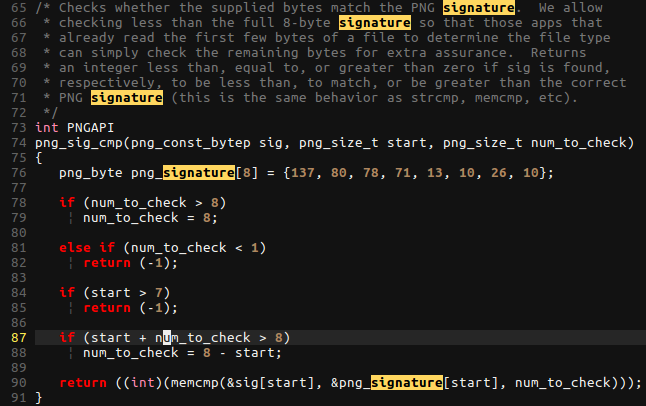
\includegraphics[scale=0.6]{/home/brandon/Desktop/IFT_194/labs/photos/signature.png}
  \caption{Lines in \texttt{png.c} that define the signature bytes of the PNG image specification. In hexadecimal format, the sequence is \texttt{89 50 4E 47 0D 0A 1A 0A}.}
  \label{fig:one}
\end{figure}
\begin{figure}
  \centering
  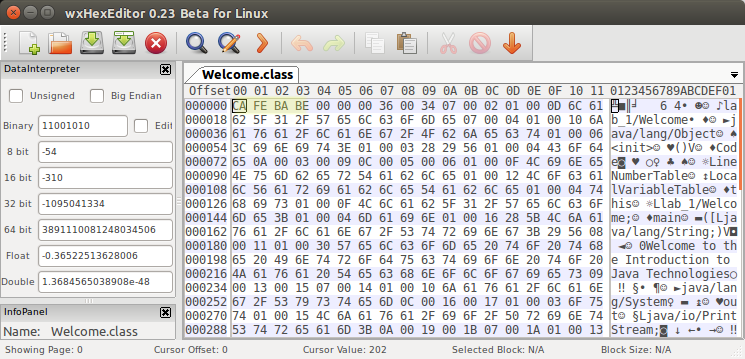
\includegraphics[scale=0.55]{/home/brandon/Desktop/IFT_194/labs/photos/class_signature.png}
  \caption{First four signature bytes of my \texttt{Welcome.class} file, generated for Lab 1.}
  \label{fig:two}
\end{figure}

\end{document}
